\documentclass[conference]{IEEEtran}
\IEEEoverridecommandlockouts
\usepackage{cite}
\usepackage{amsmath,amssymb,amsfonts}
\usepackage{graphicx}
\usepackage{textcomp}
\usepackage{xcolor}
\usepackage{tikz}
\usetikzlibrary{shapes.geometric, arrows.meta, positioning, calc, fit, backgrounds}

\tikzset{
  proc/.style={rectangle, rounded corners=2pt, draw=black!70, fill=blue!5,
               minimum height=7mm, text width=27mm, align=center, font=\scriptsize},
  term/.style={rectangle, rounded corners=8pt, draw=black!70, fill=black!8,
               minimum height=7mm, text width=25mm, align=center, font=\scriptsize},
  dec/.style={diamond, aspect=2.2, draw=black!70, fill=orange!12,
              inner sep=1pt, text width=21mm, align=center, font=\scriptsize},
  esc/.style={rectangle, rounded corners=2pt, draw=black!70, fill=red!8,
              minimum height=7mm, text width=25mm, align=center, font=\scriptsize},
  lay/.style={rectangle, rounded corners=2pt, draw=black!70, fill=blue!5,
              minimum height=7.5mm, text width=21mm, align=center, font=\scriptsize},
  mod/.style={rectangle, rounded corners=2pt, draw=black!70, fill=green!7,
              minimum height=6.5mm, text width=20mm, align=center, font=\scriptsize},
  grp/.style={rectangle, rounded corners=3pt, draw=black!45, dashed, inner sep=2.4mm},
  fl/.style={-{Latex[length=1.6mm]}, draw=black!70},
  lbl/.style={font=\scriptsize\itshape, inner sep=1.5pt},
  tier/.style={font=\scriptsize\bfseries, rotate=90, anchor=south, inner sep=1.5mm}
}

\begin{document}

\title{SHARP: A Smart Hostel Administration and Resource Platform\\
{\footnotesize Digital Workflows for Leave, Mess, Allotment, Maintenance and Laundry Services}}

\author{
\IEEEauthorblockN{Ali Ekram}
\IEEEauthorblockA{\textit{CSED, Roll No. 1024160138} \\
\textit{Thapar Institute of Engineering and Technology}\\
Patiala, India}
\and
\IEEEauthorblockN{Vaibhav Kansal}
\IEEEauthorblockA{\textit{CSED, Roll No. 1024160097} \\
\textit{Thapar Institute of Engineering and Technology}\\
Patiala, India}
\and
\IEEEauthorblockN{Riya Gupta}
\IEEEauthorblockA{\textit{CSED, Roll No. 1024160122} \\
\textit{Thapar Institute of Engineering and Technology}\\
Patiala, India}
\and
\IEEEauthorblockN{Ayush Kamboj}
\IEEEauthorblockA{\textit{CSED, Roll No. 1024160118} \\
\textit{Thapar Institute of Engineering and Technology}\\
Patiala, India}
}

\maketitle

\begin{abstract}
Hostel administration still depends on handwritten applications, physical registers and
loosely tracked complaints, which produces delays, broken room clusters, unresolved
maintenance and lost laundry. SHARP is a centralised web platform unifying five such
processes---leave and visitor passes, mess feedback, room allotment, maintenance complaints
and laundry---behind role-based workflows for students, parents, wardens, caretakers, mess
staff and laundry staff. The goal is not digitisation alone but traceability and
accountability: complaints close only on student verification, room reservations expire
automatically, laundry issues are logged against each submission so recurring problems surface
in the data, and mess feedback stays anonymous to mess staff while remaining auditable.
\end{abstract}

\begin{IEEEkeywords}
hostel management, workflow automation, role-based access control, SLA escalation,
issue reporting, web application
\end{IEEEkeywords}

\section{Introduction}
Several routine hostel processes are partially manual or lack tracking: leave approvals are
delayed, complaint status is unknown, clusters break under staggered fee payment, and laundry
losses go unrecorded. SHARP gives every participant one platform for the services their role
covers, and each module adds a mechanism the manual process lacks---a verification step, an
expiry rule or an escalation timer---rather than reproducing paperwork on a screen.

\section{Problem Statement}
Five pain points motivate the system. \textit{Leave and passes:} handwritten applications and
manual parent contact create paperwork and delay. \textit{Mess feedback:} register-based
collection discourages honesty because identity is visible. \textit{Allotment:} when cluster
members pay at different times, a partly reserved room may be taken by others, breaking
clusters. \textit{Maintenance:} complaints stay unresolved for days, progress is untrackable
and preferred slots go unhonoured. \textit{Laundry:} lost or damaged items are reported
informally if at all, so recurring problems---a particular day, batch or item type---go
unnoticed. Each is a traceability gap.

\section{Proposed System}
SHARP comprises five modules. \textit{Visitor and leave management} handles day-out, regular
and emergency requests carrying start and end time, destination, reason and emergency contact,
routed as Student $\rightarrow$ Parent verification $\rightarrow$ Warden approval
$\rightarrow$ digital pass with a unique ID shown at exit. \textit{Mess management} takes
categorised feedback on quality, hygiene, quantity, menu, timing and service plus special meal
requests such as khichdi during illness or Jain diets; feedback is anonymous to mess staff
while internal records deter abuse, and administrators see aggregates such as a weekly rise in
food-quality complaints.

\textit{Allotment} adds a temporary reservation: a cluster leader holds a room while members
complete payment, and the room advances through Available $\rightarrow$ Temporarily Reserved
$\rightarrow$ Partially Confirmed $\rightarrow$ Fully Confirmed $\rightarrow$ Allotted. The
reservation expires after a set window, say 48 hours, returning the room to the pool---which
preserves clusters without weakening the fee requirement.

\begin{figure}[!t]
\centering
\resizebox{0.70\columnwidth}{!}{%
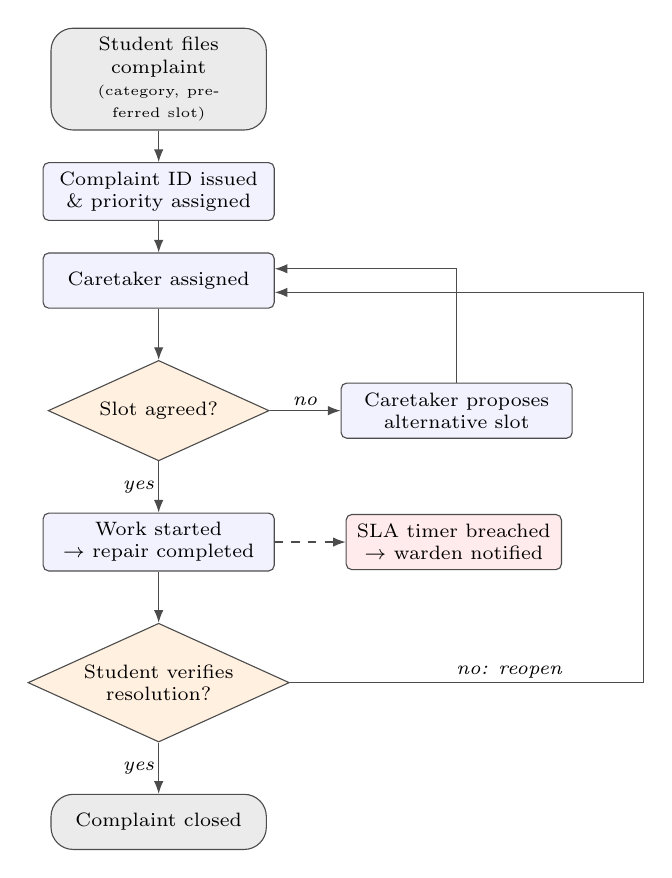
\begin{tikzpicture}[node distance=4mm]
\node[term] (a) {Student files complaint\\{\tiny(category, preferred slot)}};
\node[proc, below=of a] (b) {Complaint ID issued\\ \& priority assigned};
\node[proc, below=of b] (c) {Caretaker assigned};
\node[dec, below=6.5mm of c] (d) {Slot agreed?};
\node[proc, right=9mm of d] (e) {Caretaker proposes\\alternative slot};
\node[proc, below=6.5mm of d] (f) {Work started\\$\rightarrow$ repair completed};
\node[dec, below=6.5mm of f] (g) {Student verifies\\resolution?};
\node[term, below=6.5mm of g] (h) {Complaint closed};
\node[esc, right=9mm of f] (s) {SLA timer breached\\$\rightarrow$ warden notified};
\draw[fl] (a) -- (b);
\draw[fl] (b) -- (c);
\draw[fl] (c) -- (d);
\draw[fl] (d) -- node[lbl,above]{no} (e.west);
\coordinate (rr) at ($(e.east)+(9mm,0)$);
\draw[fl] (e.north) |- ($(c.east)+(0,1.5mm)$);
\draw[fl] (d) -- node[lbl,left]{yes} (f);
\draw[fl] (f) -- (g);
\draw[fl] (g) -- node[lbl,left]{yes} (h);
\draw[fl] (g.east) -- node[lbl,above,pos=0.62]{no: reopen} (g.east -| rr) |- ($(c.east)+(0,-1.5mm)$);
\draw[fl, dashed] (f.east) -- (s.west);
\end{tikzpicture}}
\caption{Maintenance complaint lifecycle. Closure requires student verification, and a negative
answer reopens the ticket against the same ID; an SLA timer escalates independently.}
\label{fig:complaint}
\end{figure}

\textit{Complaint management} issues an ID per maintenance report and runs the lifecycle of
Fig.~\ref{fig:complaint}, distinguished from a status field by student verification before
closure and SLA escalation to the warden. \textit{Laundry issue tracking} leaves the physical
process unchanged; a student reports a problem against a submission---missing, damaged, wrong
or stained items, or a delay---logged with a timestamp and category, and aggregated reports
let administrators spot recurring issues such as an item type or day with an unusual failure
rate.

\section{System Architecture}
SHARP uses a layered architecture (Fig.~\ref{fig:arch}): a role-specific interface layer, an
application and REST API layer carrying authentication and authorisation, a business logic
layer holding the five modules, a persistence layer, and optional external services. Access
control is cross-cutting---every sensitive endpoint checks both identity and permission, so a
student cannot reach administrative dashboards, parent records or the identity behind
anonymous feedback---and modules stay separable, so one can change without redesigning the
application.

\begin{figure}[!t]
\centering
\resizebox{0.84\columnwidth}{!}{%
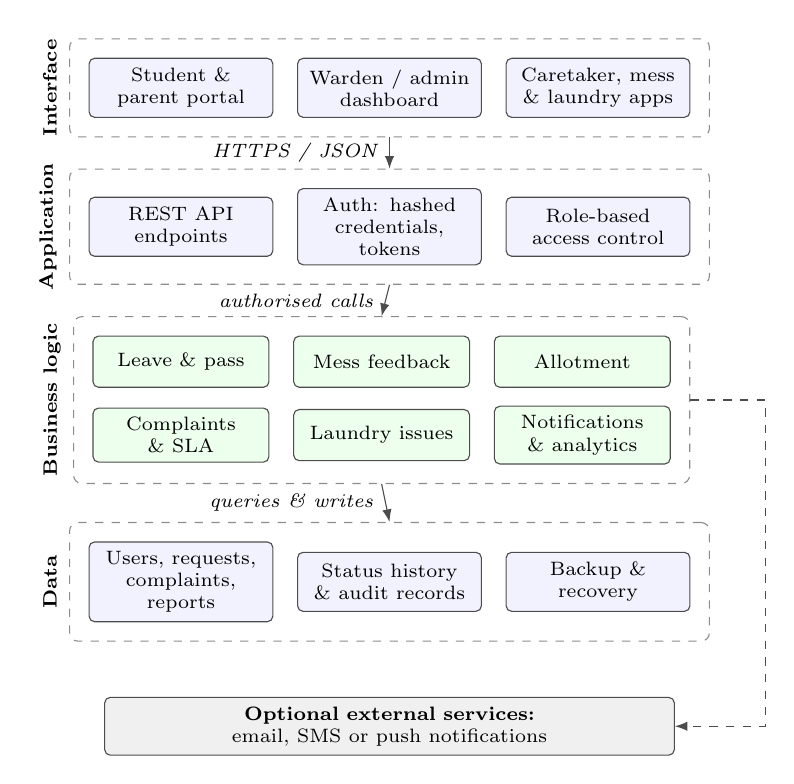
\begin{tikzpicture}[node distance=3mm]
\node[lay] (u1) {Student \& parent portal};
\node[lay, right=of u1] (u2) {Warden / admin dashboard};
\node[lay, right=of u2] (u3) {Caretaker, mess \& laundry apps};
\begin{scope}[on background layer]
\node[grp, fit=(u1)(u2)(u3)] (P) {};
\end{scope}
\node[tier] at (P.west) {Interface};

\node[lay, below=10mm of u1] (a1) {REST API endpoints};
\node[lay, right=of a1] (a2) {Auth: hashed\\credentials, tokens};
\node[lay, right=of a2] (a3) {Role-based access control};
\begin{scope}[on background layer]
\node[grp, fit=(a1)(a2)(a3)] (A) {};
\end{scope}
\node[tier] at (A.west) {Application};

\node[mod, below=10mm of a1] (m1) {Leave \& pass};
\node[mod, right=of m1] (m2) {Mess feedback};
\node[mod, right=of m2] (m3) {Allotment};
\node[mod, below=2.5mm of m1] (m4) {Complaints \& SLA};
\node[mod, right=of m4] (m5) {Laundry issues};
\node[mod, right=of m5] (m6) {Notifications \& analytics};
\begin{scope}[on background layer]
\node[grp, fit=(m1)(m2)(m3)(m4)(m5)(m6)] (B) {};
\end{scope}
\node[tier] at (B.west) {Business logic};

\node[lay, below=10mm of m4] (d1) {Users, requests,\\complaints, reports};
\node[lay, right=of d1] (d2) {Status history\\\& audit records};
\node[lay, right=of d2] (d3) {Backup \&\\recovery};
\begin{scope}[on background layer]
\node[grp, fit=(d1)(d2)(d3)] (D) {};
\end{scope}
\node[tier] at (D.west) {Data};

\node[rectangle, rounded corners=2pt, draw=black!70, fill=black!6, font=\scriptsize,
      align=center, minimum height=6.5mm, below=7mm of D.south, anchor=north,
      text width=70mm] (x)
  {\textbf{Optional external services:} email, SMS or push notifications};

\draw[fl] (P.south) -- node[lbl,left,xshift=-1mm]{HTTPS / JSON} (A.north);
\draw[fl] (A.south) -- node[lbl,left,xshift=-1mm]{authorised calls} (B.north);
\draw[fl] (B.south) -- node[lbl,left,xshift=-1mm]{queries \& writes} (D.north);
\draw[fl, dashed] (B.east) -| ($(D.east)+(7mm,0)$) |- (x.east);
\end{tikzpicture}}
\caption{Layered architecture. Each block names a role rather than a product, so the stack can
be fixed later; external services stay optional.}
\label{fig:arch}
\end{figure}

\subsection{Technology and Language Flexibility}
The layers are specified by responsibility, not by product, so the implementation language and
framework will be decided at the time of building, once the team has weighed hosting, library
maturity and its own familiarity. A JavaScript stack---React with Tailwind CSS, Node.js with
Express, MongoDB and token authentication---is a proven candidate and is used for costing, but
any stack offering a REST-capable framework, a managed database, secure token authentication
and a test framework satisfies the design. Deferring the choice costs nothing: no workflow
rule, role definition or metric depends on a particular language.

\section{Requirements}
Students file leave requests, track approvals, hold passes, submit anonymous feedback and meal
requests, raise and reopen complaints with preferred slots, and report lost or damaged laundry.
Parents act on leave notifications; wardens approve leave, manage rooms and clusters, assign
caretakers and view analytics; caretakers accept assignments, propose slots and update status;
mess staff work within their feedback queue and laundry staff respond to logged issues.
Non-functionally, operations should complete within seconds at hostel-scale load, passwords
must be hashed, parent approval tokens must resist unauthorised use, the service must stay
available outside administrative hours, and the schema should admit further hostels without
redesign.

\section{Feasibility and Cost}
The system needs no special hardware, and the toolchain is free or open source: the prototype
costs roughly \textrm{INR}\,0--3{,}500, dominated by optional hosting, domain and SMS. It is
operationally feasible because it adds reporting on top of workflows students already
understand. Delivery is phased---authentication and roles, then leave, complaints, mess,
allotment, laundry issue tracking, and finally notifications and deployment---so a working
minimum viable product exists even if later phases are unfinished.

\section{Risks and Success Metrics}
Risks and mitigations are: unauthorised access, met by role-based authentication; forged
parent approval, met by secure tokens plus warden verification; abuse of anonymous feedback,
met by rate limits and audit records; premature loss of a reservation, met by expiry rules and
transactional validation; and disputed laundry loss, met by timestamped reports tied to a
submission. Success is measured by the fall in paper applications, average leave approval and
complaint resolution times, share of complaints closed within SLA, reopen count, laundry
issues reported per month and reservation conflicts avoided.

\section{Conclusion}
SHARP turns five disconnected hostel processes into one auditable platform, adding
verification, expiry and escalation mechanisms rather than merely replacing paper, and is
feasible technically, economically and operationally as a course project.

\end{document}
